\documentclass[11pt,a4paper]{article}
\usepackage[T1]{fontenc}
\usepackage[utf8]{inputenc}
\usepackage{lmodern,microtype,amsmath,amssymb,mathtools,bm}
\usepackage[a4paper,left=25mm,right=25mm,top=24mm,bottom=24mm]{geometry}
\usepackage{booktabs,array,tabularx,enumitem,xcolor,tikz,pgfplots,fancyhdr}
\usepackage[most]{tcolorbox}
\usepackage[pdfauthor={},pdfsubject={},pdfcreator={},pdftitle={Quantum Memory Certification: A Finite Storage-Gap Bound},colorlinks=true,linkcolor=blue!45!black,urlcolor=blue!45!black]{hyperref}
\usetikzlibrary{arrows.meta,positioning,calc}
\pgfplotsset{compat=1.18}
\definecolor{ink}{HTML}{17334B}
\definecolor{accent}{HTML}{247B91}
\definecolor{pale}{HTML}{EEF5F7}
\definecolor{warm}{HTML}{AA642C}
\setlength{\parindent}{0pt}
\setlength{\parskip}{4pt plus 1pt}
\setlength{\emergencystretch}{1.8em}
\linespread{1.035}
\setlist{nosep,leftmargin=1.5em}
\pagestyle{fancy}
\fancyhf{}
\fancyhead[L]{\small\sffamily\color{ink}QUANTUM MEMORY CERTIFICATION}
\fancyhead[R]{\small\sffamily EXPLANATORY REPORT}
\fancyfoot[C]{\small\thepage}
\renewcommand{\headrulewidth}{0.3pt}
\setlength{\headheight}{15pt}
\newtcolorbox{keybox}[1][]{colback=pale,colframe=accent,boxrule=0.5pt,arc=1mm,left=3mm,right=3mm,top=2mm,bottom=2mm,#1}
\newcommand{\Tr}{\operatorname{Tr}}
\newcommand{\rank}{\operatorname{rank}}
\newcommand{\E}{\mathbb E}
\newcommand{\ket}[1]{\lvert #1\rangle}
\newcommand{\bra}[1]{\langle #1\rvert}
\newcommand{\ip}[2]{\langle #1\mid #2\rangle}
\newcommand{\pgm}{P_{\mathrm{pgm}}}
\newcommand{\popt}{P_{\mathrm{opt}}}
\newcommand{\pguess}{p_{\mathrm{guess}}}
\newcommand{\Dmap}{\mathcal D}
\newcommand{\HH}{\mathsf H}
\newcommand{\XX}{\mathsf X}
\newcommand{\YY}{\mathsf Y}
\newcommand{\ZZ}{\mathsf Z}
\newcommand{\normn}[2]{\lVert #1\rVert_{#2,\mathrm n}}
\newcommand{\newsection}[1]{\section{#1}}
\begin{document}
\thispagestyle{plain}
{\sffamily\color{accent}\small EXPLANATORY REPORT\par}
\vspace{3mm}
{\LARGE\bfseries\color{ink}Quantum Memory Certification\par}
\vspace{2mm}
{\Large A finite storage-gap bound\par}
\vspace{4mm}

\section{The question and the answer}
A device receives a string of qubits. Each qubit encodes a classical bit in one of two incompatible measurement bases. The device may process the entire collection, measure part of it, and keep any classical record it wants. Only after a prescribed storage cut does it learn the bases. It must then recover the entire hidden bit string.

Keeping the original quantum states would allow perfect readout once the bases arrive. A premature measurement generally loses the option of choosing the right measurement later. The question is how much this loss matters when the device retains almost, but not quite, enough quantum memory for the whole input.

Let the integer $k\geq1$ count the input qubits and let $d_Q\geq1$ be the dimension of all quantum information that survives the cut and is later accessible. For a fixed encoder, $\pguess$ is the best probability of exact whole-string recovery over all allowed decoders, averaged over the random bits, bases, and processing outcomes. Every encoder obeys the finite, unsmoothed bound
\begin{keybox}
\begin{equation}\label{eq:main}
\pguess\leq\min\left\{1,\left(\frac{d_Q}{2^k}\right)^{1/6}\right\}.
\end{equation}
For at most $m$ retained qubits, with $d_Q\leq2^m$ and $0\leq m\leq k$, the missing-qubit gap $t=k-m$ gives
\begin{equation}\label{eq:gap}
\pguess\leq2^{-t/6}.
\end{equation}
These are bounds for exact recovery of the whole string, allowing joint processing and unlimited classical storage.
\end{keybox}

The dependence on $t$ is the central feature. To force ideal cheating probability to at most a fixed $\delta\in(0,1)$, it suffices to supply $\lceil6\log_2(1/\delta)\rceil$ more qubits than the device can retain. This sufficient gap has no additional dependence on the stored block size. An explicit strategy shows that the logarithmic order cannot be improved within this ideal test, although the constants remain unmatched.

Rank-sensitive finite refinements give one-retained-qubit guessing caps $C_3\simeq0.743718$, $C_4\simeq0.642943$ and $C_5\simeq0.556840$ for three, four and five inputs, with arbitrary joint encoders and unlimited classical records. Their averaged PGM optima are exactly $9/16$, $27/64$ and $81/256$. A separate construction shows that the collision statistic used in the general proof has sharp exponent $1/3$ in the memory deficit. Thus this finite improvement does not improve the uniform guessing exponent $1/6$; a stronger general result needs information beyond that statistic and its square-root conversion.

A direct-discrimination follow-up adds exact decoder certificates for two specified encoders and proves that a diagonal dual ansatz loses even the known decay scale on the asymptotic obstruction family. These are methodological results; these specified-encoder certificates improve neither the global caps nor the uniform exponent.

A second layer uses a computationally secure preparation protocol to let a verifier conduct the test using classical interaction. Under its precise assumptions, the false-acceptance bound becomes
\begin{equation}\label{eq:compiled-front}
P_{\mathrm{accept}}\leq\min\{1,\eta_{\mathrm{prep}}+2^{-t/6}\},
\end{equation}
where $\eta_{\mathrm{prep}}$ is the remote-state-preparation simulation error. Write $\varepsilon\in(0,1)$ for a target total false-acceptance probability, while $\delta$ denotes a target ideal guessing probability. The ideal bound is unconditional; the classical realization inherits a quantum-hardness assumption and applies to the efficient adversaries in its preparation guarantee.

The report develops the experiment first, then proves the finite bound, explains the conditional realization, and tests its boundaries. Exact recovery, error-tolerant acceptance, and erasures are treated separately because they certify different storage restrictions. A final application shows how the same guessing task can imply a processing budget under a specified fully noisy device model.

\newsection{The experiment and its information budget}
\subsection{Two bases, one hidden string}
The computational basis is $\{\ket0,\ket1\}$, where these two unit vectors are orthogonal. The second basis is $\{\ket+,\ket-\}$, with
\[
\ket+=\frac{\ket0+\ket1}{\sqrt2},\qquad
\ket-=\frac{\ket0-\ket1}{\sqrt2}.
\]
The Hadamard matrix $\HH=2^{-1/2}\left(\begin{smallmatrix}1&1\\1&-1\end{smallmatrix}\right)$ maps the first basis to the second. Independently uniform strings $X,\Theta\in\{0,1\}^k$ specify bit values and bases. The supplied state is
\[
\ket{x}_\theta=U_\theta\ket{x},\qquad
U_\theta=\bigotimes_{i=1}^k \HH^{\theta_i}.
\]
This four-state encoding is called BB84. A state is described by a density operator: a positive matrix $\rho$ with $\Tr\rho=1$, where $\Tr$ sums diagonal entries. Write $I_k$ for the identity in dimension $k$. For either basis, averaging over the uniformly random bit gives $I_2/2$, so the input alone does not reveal the selected basis.

\begin{center}
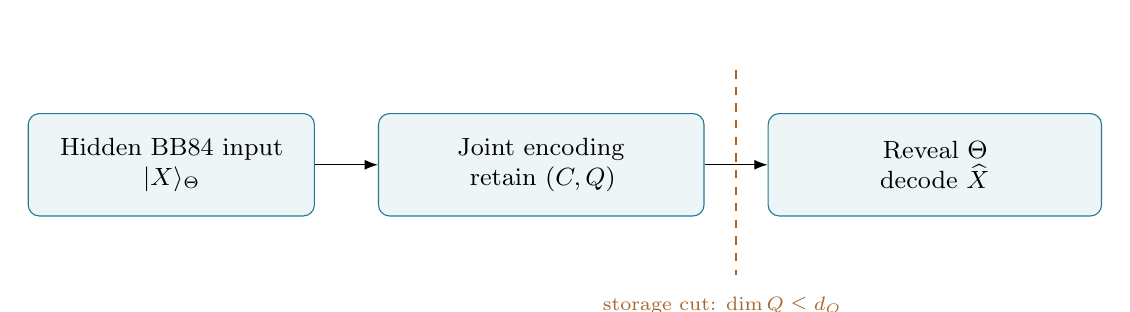
\begin{tikzpicture}[font=\small,>=Latex]
\node[draw=accent,rounded corners,fill=pale,text width=34mm,align=center,minimum height=13mm] (a) {Hidden BB84 input\\$\ket X_\Theta$};
\node[draw=accent,rounded corners,fill=pale,text width=39mm,align=center,minimum height=13mm,right=8mm of a] (b) {Joint encoding\\retain $(C,Q)$};
\node[draw=accent,rounded corners,fill=pale,text width=40mm,align=center,minimum height=13mm,right=8mm of b] (c) {Reveal $\Theta$\\decode $\widehat X$};
\draw[->] (a)--(b);\draw[->] (b)--(c);
\draw[dashed,warm,thick] ($(b.east)+(4mm,12mm)$)--($(b.east)+(4mm,-14mm)$);
\node[font=\scriptsize,text=warm,below=9mm of b,xshift=23mm] {storage cut: $\dim Q\leq d_Q$};
\end{tikzpicture}
\end{center}

\subsection{What the encoder and decoder may do}
Before learning $\Theta$, the device applies any quantum instrument: a joint operation with classical outcome $C$ and retained quantum output $Q$. It may measure, transform, or discard subsystems, with no size bound on $C$. The dimension restriction counts every quantum system accessible after the cut, including remotely held ancillas and previously correlated references.

After disclosure, the decoder uses a measurement depending on $(C,\Theta)$. Its positive operators $M_x$ sum to the identity and form a positive operator-valued measure (POVM); on state $\rho$, outcome $x$ has probability $\Tr(M_x\rho)$. Exact success is $\widehat X=X$. The ideal analysis permits arbitrary computational power and fresh, uncorrelated decoding workspace, which can be absorbed into the POVM. An environment returned later must be counted in $Q$.

\begin{center}\small
\begin{tabularx}{\linewidth}{@{}lX@{}}\toprule
Symbol & Meaning \\\midrule
$k,d=2^k$ & Input qubit count and Hilbert-space dimension.\\
$d_Q,m$ & Retained quantum dimension and a qubit budget with $d_Q\leq2^m$.\\
$t=k-m$ & Missing-qubit gap, used when $0\leq m\leq k$.\\
$X,\Theta,\widehat X$ & Hidden bits, later-revealed bases, and returned guess.\\
$C,Q$ & Classical record and all charged persistent quantum information.\\
\bottomrule\end{tabularx}\end{center}
Logarithms written as $\log_2$ have base two; $\ln$ denotes the natural logarithm. The waiting duration is a separate experimental parameter. For a classical hidden variable, conditional min-entropy is the operational quantity
\[
H_{\min}(X\mid CQ\Theta)=-\log_2\pguess(X\mid CQ\Theta).
\]
Thus \eqref{eq:gap} also states $H_{\min}(X\mid CQ\Theta)\geq t/6$, without a smoothing parameter or asymptotic remainder.

\newsection{A strategy that makes the gap tangible}
\subsection{One stored qubit and one premature measurement}
For $k=2$ and $m=1$, store the first qubit untouched. Once its basis is revealed, measure it correctly. For the second qubit, use the intermediate measurement axis
\[
B=\frac{\XX+\ZZ}{\sqrt2},\qquad
\XX=\begin{pmatrix}0&1\\1&0\end{pmatrix},\quad
\ZZ=\begin{pmatrix}1&0\\0&-1\end{pmatrix}.
\]
The two eigenvectors can be chosen as
\[
\ket{b_0}=\cos(\pi/8)\ket0+\sin(\pi/8)\ket1,\qquad
\ket{b_1}=-\sin(\pi/8)\ket0+\cos(\pi/8)\ket1.
\]
For input vector $\ket\psi$, outcome $c$ has probability $|\ip{b_c}{\psi}|^2$; the bra $\bra{b_c}$ is the conjugate transpose of the ket $\ket{b_c}$. Record $c\in\{0,1\}$ and return it as the bit guess in either announced basis. For example,
\[
|\ip{b_0}{0}|^2=|\ip{b_0}{+}|^2
=\beta,\qquad
\beta=\cos^2(\pi/8)=\frac{1+1/\sqrt2}{2}\simeq0.853553.
\]
The same success probability holds for bit one and the other outcome. This intermediate-axis measurement is often called the Breidbart measurement. Measuring in one of the two encoding bases instead would give average bit success $3/4$, which is lower.

The stored bit is recovered perfectly, so this one-qubit-memory strategy achieves whole-string success $\beta$. The universal upper bound is $2^{-1/6}\simeq0.890899$.

\subsection{Store a block and measure the remainder}
For integer $0\leq m\leq k$, store any $m$ positions and apply the intermediate measurement to each of the remaining $t=k-m$ positions. The product source and this product strategy yield
\begin{equation}\label{eq:witness}
P_{\mathrm{ach}}=\beta^t.
\end{equation}
This supplies a lower bound on the optimal cheating probability; the theorem supplies the upper bound:
\begin{equation}\label{eq:bracket}
\beta^t\leq P^*_{k,m}\leq2^{-t/6}.
\end{equation}
Here $P^*_{k,m}$ is the optimum over both encoders and decoders. A measurement record helps, but it does not preserve the ability to choose an arbitrary measurement after disclosure.

At full memory, $m=k$, storing every input gives success one. At zero quantum memory, the bound is $2^{-k/6}$ and the displayed strategy achieves $\beta^k$. The constants are examined in Section~\ref{sec:overhead}.

\newsection{A proof representation that preserves the memory budget}
The proof first resolves a general strategy into pure conditional branches, where memory dimension limits Schmidt rank. It then converts guessing into an averaged quadratic expression and uses the rank restriction to bound that expression.
\subsection{Delay the verifier's measurement}
Consider a more general experiment. Before the basis is chosen, the verifier holds a $k$-qubit register $A$, jointly in any state $\rho_{ACQ}$ with the device's records. Being classical on $C$ means a mixture of distinguishable labels $c$ and their conditional quantum states. Assume $\dim Q\leq d_Q$. Select $\Theta$ uniformly and independently of this state, then measure $A$ in basis $\Theta$. Call the result $X$. The device, given $(C,Q,\Theta)$, guesses $X$.

The theorem will hold in this arbitrary-state model. It includes the original preparation task by a delayed-measurement representation. Start with $k$ copies of
\[
\ket\Phi_{AB}=\frac{\ket{00}+\ket{11}}{\sqrt2}.
\]
For the full block write $\ket{\Phi_d}=d^{-1/2}\sum_z\ket z_A\ket z_B$. The identity
\[
(\bra xU_\theta^\dagger\otimes I)\ket{\Phi_d}
=d^{-1/2}U_\theta^*\ket x
=d^{-1/2}\ket x_\theta
\]
uses the reality of the BB84 matrices. It shows that each outcome $x$ has probability $1/d$ and prepares the corresponding state on $B$. If $\mathcal E$ is the device's encoding instrument, its action on $B$ commutes with the measurement on $A$. Uniformly choosing $\theta$ therefore gives the joint output
\[
\frac1{d^2}\sum_{x,\theta}\ket{x,\theta}\bra{x,\theta}
\otimes\mathcal E(\ket x_\theta\bra x_\theta).
\]
This is exactly the original source and encoder, including their probability weights. The verifier's measurement can be placed after the storage cut in the analysis. The physical classical verifier is implemented separately by the preparation protocol below.

In the original preparation task, $(X,\Theta)$ is uniform by construction. In the arbitrary-state model, $X$ need not be uniform, even conditioned on a classical branch. The proof must retain its actual probability weights.

\subsection{Use pure branches without adding quantum memory}
Condition on $C=c$ and decompose the remaining state into normalized pure states:
\[
\rho_{AQ}^{c}=\sum_j p(j\mid c)\ket{\psi_{cj}}\bra{\psi_{cj}}.
\]
For an upper bound on guessing, give the hypothetical decomposition label $j$ to the decoder as extra classical information. A decoder may ignore it, so this can only increase optimal success. No additional quantum system is supplied. Because $\Theta$ is independent of the premeasurement state, revealing $(c,j)$ does not bias its distribution.

It remains to prove the same bound for each pure branch $\ket\psi_{AQ}$. Its Schmidt decomposition has the form
\begin{equation}\label{eq:schmidt}
\ket\psi=\sum_{j=1}^{r}\sqrt{\lambda_j}\ket{a_j}_A\ket{b_j}_Q,
\qquad\lambda_j>0,\quad\sum_j\lambda_j=1.
\end{equation}
Here both vector families are orthonormal, and the Schmidt rank obeys $r\leq\min(d_Q,d)$. The reduced state $\rho=\Tr_Q\ket\psi\bra\psi$ has exactly these $r$ nonzero eigenvalues. The partial trace $\Tr_Q$ discards $Q$ while preserving every measurement probability on $A$.

\begin{keybox}
The rank restriction applies to a pure conditional branch. An arbitrary mixed $\rho_{AQ}$ can have $\rho_A=I_d/d$ even when $Q$ is one-dimensional. Giving away a quantum purification would change the charged memory; revealing a classical decomposition label does not.
\end{keybox}

\newsection{Control every decoder through one specified measurement}
For a fixed pure branch and announced basis, the possible outcomes define a quantum state-discrimination problem. We first prove a general comparison that avoids optimizing the decoder explicitly.

Let $\{\sigma_x\}$ be positive, subnormalized operators on $Q$, with
\[
S=\sum_x\sigma_x,\qquad\Tr S=1.
\]
The operator $\sigma_x=p_x\rho_x$ combines a label's probability $p_x$ and its normalized conditional state $\rho_x$, so $\Tr\sigma_x=p_x$. For a POVM $\{M_x\}$, success is $\sum_x\Tr(M_x\sigma_x)$; write $\popt$ for its supremum over all POVMs. The square-root, or pretty-good, measurement has effects $S^{-1/2}\sigma_xS^{-1/2}$ on the support of $S$: the span of its eigenvectors with nonzero eigenvalues. Outside that support it can be completed arbitrarily, because the ensemble never occupies it. Its success is
\begin{equation}\label{eq:pgm-def}
\pgm=\sum_x\Tr(\sigma_xS^{-1/2}\sigma_xS^{-1/2}).
\end{equation}
Inverse powers act only on this support, so zero eigenvalues cause no ambiguity.

For any decoder, define Hermitian positive operators
\[
A_x=S^{-1/4}\sigma_xS^{-1/4},\qquad
B_x=S^{1/4}M_xS^{1/4}.
\]
Cyclicity of trace gives $\sum_x\Tr(A_xB_x)=\sum_x\Tr(M_x\sigma_x)$. Cauchy--Schwarz for the direct sum of the matrix spaces gives
\[
\left(\sum_x\Tr M_x\sigma_x\right)^2
\leq\left(\sum_x\Tr A_x^2\right)
     \left(\sum_x\Tr B_x^2\right).
\]
The first factor equals \eqref{eq:pgm-def}. For the second, $\sum_xB_x=S^{1/2}$ and positivity implies $\Tr(B_xB_y)\geq0$. Consequently,
\[
1=\Tr S=\Tr\left(\sum_x B_x\right)^2
\geq\sum_x\Tr B_x^2.
\]
Taking the supremum over all decoding POVMs proves
\begin{keybox}
\begin{equation}\label{eq:discrimination}
\popt^2\leq\pgm,\qquad\popt\leq\sqrt{\pgm}.
\end{equation}
\end{keybox}
This established inequality controls every decoder through the tractable quantity $\pgm$; the square-root measurement itself need not be optimal.

\newsection{Why the square root of a marginal appears}
Return to the Schmidt decomposition \eqref{eq:schmidt}. Set $R=\sqrt\rho$, where powers are taken spectrally: an eigenvalue $\lambda$ of $\rho$ becomes $\sqrt\lambda$ in $R$. For a fixed basis string $\theta$, measuring $A$ gives the subnormalized vector
\[
\ket{v_x}=\sum_{j=1}^r\sqrt{\lambda_j}\ip{x_\theta}{a_j}\ket{b_j},
\qquad\sigma_x=\ket{v_x}\bra{v_x}.
\]
Its squared norm is the actual probability of $x$. Summing over all basis vectors gives
\[
S=\sum_x\sigma_x=\sum_{j=1}^r\lambda_j\ket{b_j}\bra{b_j},
\]
which is independent of $\theta$. Hence
\begin{align*}
\bra{v_x}S^{-1/2}\ket{v_x}
&=\sum_{j=1}^r\sqrt{\lambda_j}|\ip{x_\theta}{a_j}|^2\\
&=\bra{x_\theta}R\ket{x_\theta}.
\end{align*}
For a rank-one $\sigma_x$, its contribution to \eqref{eq:pgm-def} is the square of this overlap. Therefore the exact identity is
\begin{equation}\label{eq:pgm-id}
\pgm(\theta)=\sum_x\bra{x_\theta}R\ket{x_\theta}^{\!2}.
\end{equation}
The diagonal entries are real and nonnegative because $R$ is positive. There is no additional division by an outcome probability and no uniform-outcome assumption.

\subsection{The two-qubit example inside the proof}
In the earlier strategy, condition on the intermediate-axis measurement result $c$. The delayed-measurement state is a Bell pair on $A_1Q$ tensored with $\ket{b_c}$ on $A_2$. Thus
\[
\rho=\frac{I_2}{2}\otimes\ket{b_c}\bra{b_c},\qquad
R=\frac{I_2}{\sqrt2}\otimes\ket{b_c}\bra{b_c}.
\]
Its rank is two. In either basis, the second register's probabilities are $\beta$ and $1-\beta$. Summing \eqref{eq:pgm-id} over the first bit and the second bit yields
\[
\pgm=\beta^2+(1-\beta)^2=\frac34.
\]
For this branch the optimal decoder attains $\beta$: the first bit can be read perfectly and the second is best guessed by its larger conditional probability. The proof chain gives
\[
0.853553\simeq\beta\leq\sqrt{3/4}\simeq0.866025
\leq2^{-1/6}\simeq0.890899.
\]
The example makes the slack introduced by the inequalities visible.

\newsection{Average the bases using Pauli coordinates}
\subsection{Measurement averaging as dephasing}
Dephasing in a basis deletes off-diagonal matrix entries in that basis. Write these maps as $\Delta_Z$ and $\Delta_X$ for the computational and Hadamard bases, and define
\[
\mathcal T=\frac{\Delta_Z+\Delta_X}{2}.
\]
For one basis, the squared diagonal sum in \eqref{eq:pgm-id} equals $\Tr[R\Delta(R)]$. Independent choices of the $k$ bases therefore give
\begin{equation}\label{eq:average}
\E_\Theta\pgm(\Theta)=\Tr\big[R\mathcal T^{\otimes k}(R)\big].
\end{equation}
This product of averaging maps comes from the random basis choices. It imposes no product structure on $R$, the encoder, or the decoder.

The Pauli matrices $I_2,\XX,\YY,\ZZ$, with
$\YY=\left(\begin{smallmatrix}0&-i\\i&0\end{smallmatrix}\right)$, form an orthogonal operator basis under $\Tr(A^\dagger B)$. The identity component survives either dephasing, each of the $x,z$ components survives half the time, and the $y$ component is removed:
\begin{center}\small
\begin{tabular}{@{}lrrrr@{}}\toprule
Map eigenvalue on & $I_2$ & $\XX$ & $\YY$ & $\ZZ$\\\midrule
$\mathcal T$ & $1$ & $1/2$ & $0$ & $1/2$\\
$\Dmap_{1/2}$ & $1$ & $1/2$ & $1/2$ & $1/2$\\\bottomrule
\end{tabular}\end{center}
Here the depolarizing map on a single qubit, for $0\leq\eta\leq1$, is
\[
\Dmap_\eta(A)=\eta A+(1-\eta)\Tr(A)I_2/2.
\]

\subsection{A comparison of quadratic forms}
Expand $R=\sum_P a_PP$ in $k$-qubit Pauli words, with $a_P=d^{-1}\Tr(PR)$. A word is a tensor product of the four Pauli matrices; its weight $w(P)$ counts nonidentity factors. Hermiticity makes $a_P$ real, and $\Tr(PP')=d$ when $P=P'$ and zero otherwise. Each term of the quadratic form is therefore $d a_P^2$ times the map's eigenvalue.

A word containing $\YY$ has $\mathcal T$ eigenvalue zero. Any other word has eigenvalue $2^{-w(P)}$, equal to its depolarizing eigenvalue. Term by term,
\begin{align}
\Tr[R\mathcal T^{\otimes k}(R)]
&\leq\Tr[R\Dmap_{1/2}^{\otimes k}(R)]\notag\\
&=\Tr\left[\Dmap_{1/\sqrt2}^{\otimes k}(R)^2\right].\label{eq:depolarize}
\end{align}
The equality uses self-adjointness and $\Dmap_\eta\Dmap_\zeta=\Dmap_{\eta\zeta}$. The comparison is between quadratic forms, rather than an ordering by completely positive maps. Depolarization is used to analyse the basis average; its parameter is a proof parameter, separate from physical noise in a device.

\newsection{The dimension-sensitive step and the finite theorem}
\subsection{A standard tensor-power norm inequality}
For an operator on a $d=2^k$ dimensional space, define the normalized Schatten norm
\[
\normn{A}{p}=\left(d^{-1}\Tr|A|^p\right)^{1/p},
\qquad |A|=\sqrt{A^\dagger A}.
\]
All other traces in this report are ordinary, unnormalized traces. In particular, a density operator satisfies $\Tr\rho=1$, whereas $d^{-1}\Tr I_d=1$.

The substantial standard input to the proof is qubit hypercontractivity. For Hermitian $A$, $1\leq p\leq2\leq q<\infty$, and
$0\leq\eta\leq\sqrt{(p-1)/(q-1)}$, it states
\begin{equation}\label{eq:hc}
\normn{\Dmap_\eta^{\otimes k}(A)}{q}\leq\normn{A}{p}.
\end{equation}
It says that sufficient damping of the Pauli components controls a stronger norm by a weaker one, with a constant independent of the number of qubits. Its tensor-power scope makes it applicable to entangled operators across the entire block.

\subsection{Keep the normalization factor}
Choose $p=3/2$, $q=2$, and $\eta=1/\sqrt2$. Equations \eqref{eq:average}--\eqref{eq:depolarize} imply
\begin{align}
\E_\Theta\pgm(\Theta)
&\leq d\,\normn{\Dmap_{1/\sqrt2}^{\otimes k}(R)}{2}^{2}\notag\\
&\leq d\,\normn{R}{3/2}^{2}\notag\\
&=d^{-1/3}\big(\Tr\rho^{3/4}\big)^{4/3}.\label{eq:hc-use}
\end{align}
The factor $d^{-1/3}$ follows from $d(d^{-1})^{4/3}$. Dropping this factor would destroy the storage-gap dependence.

The $r$ nonzero eigenvalues of $\rho$ sum to one. Concavity gives
\[
\frac1r\sum_{j=1}^r\lambda_j^{3/4}
\leq\left(\frac1r\sum_{j=1}^r\lambda_j\right)^{3/4},
\quad\text{hence}\quad\Tr\rho^{3/4}\leq r^{1/4}.
\]
Thus $\E\pgm\leq(r/d)^{1/3}$. Finally, use \eqref{eq:discrimination} and Cauchy--Schwarz for the classical basis average:
\begin{equation}\label{eq:finish}
\E_\Theta\popt(\Theta)
\leq\E_\Theta\sqrt{\pgm(\Theta)}
\leq\sqrt{\E_\Theta\pgm(\Theta)}
\leq(r/d)^{1/6}\leq(d_Q/d)^{1/6}.
\end{equation}
This holds on every refined pure branch. Averaging those branch bounds and removing the extra label returns the original mixed-state experiment. General classical records use the same conditional-state average; there is no alphabet-size penalty. Adding the trivial probability bound one proves \eqref{eq:main}, including non-power-of-two $d_Q$.

\subsection{A globally certified improvement for three inputs}
For $k=3$ and $d_Q=2$, every pure branch has positive $R=\sqrt\rho$ with $\rank R\le2$ and $\Tr R^2=1$. Put $t_0=(\Tr R)^2\le2$ and let $S_1$ be the sum of $(\Tr RP)^2$ over the nine weight-one Pauli words, including those containing $\YY$. Ordinary Pauli orthogonality gives $\sum_P(\Tr RP)^2=8$. The BB84 averaging map has multiplier at most $1/2$ on weight one and at most $1/4$ on all higher weights. Hence
\begin{equation}
Q:=\Tr[R\mathcal T^{\otimes3}(R)]
\le\frac18\left[t_0+\frac12S_1+\frac14(8-t_0-S_1)\right]
=\frac14+\frac{3t_0+S_1}{32}.
\label{eq:finite-purity-relaxation}
\end{equation}
The additional rank-sensitive constraint is $S_1\le t_0+2$. Here is an exact two-copy proof. For a normalized bipartite state $\sigma_{UV}$, the swap operators $F_U,F_V$ commute and have eigenvalues $\pm1$. Thus $(I-F_U)(I-F_V)\ge0$, and its expectation in $\sigma_{UV}^{\otimes2}$ gives
\[
\Tr\sigma_U^2+\Tr\sigma_V^2\le1+\Tr\sigma_{UV}^2.
\]
Applying this first to $AB|C$ and then to $A|B$ yields $\sum_{i=1}^3\Tr\sigma_i^2\le2+\Tr\sigma^2$. For $\sigma=R/\Tr R$, the Bloch identity therefore gives
\[
S_1=t_0\left(2\sum_i\Tr\sigma_i^2-3\right)\le t_0+2.
\]
Substitution in \eqref{eq:finite-purity-relaxation} proves $Q\le5/16+t_0/8\le9/16$. This is a global outer certificate for all positive rank-two $R$, not a search over a selected encoder family. It is tight as a PGM bound: $R=(I/\sqrt2)\otimes\ket b\bra b\otimes\ket b\bra b$ attains $Q=9/16$ for a pure real qubit state $\ket b$.

The established finite-alphabet discrimination inequality sharpens the square-root conversion for eight outcomes:
\[
\pgm(\theta)\ge p_\theta^2+\frac{(1-p_\theta)^2}{7},
\qquad p_\theta=\popt(\theta).
\]
It permits nonuniform probabilities and arbitrary POVMs. Convexity permits averaging over the bases, so $p^2+(1-p)^2/7\le9/16$ for $p=\E p_\Theta\ge1/8$. Solving on this interval and averaging the pure-branch refinement gives
\begin{keybox}
\[
\frac{3+2\sqrt2}{8}\le P^*_{3,1}\le
C_3:=\frac{2+7\sqrt2}{16}=0.743718433538229\ldots.
\]
The left side is the store-and-Breidbart strategy, $0.728553390593273762\ldots$. The prior normalized spectral reduction followed by the same discrimination inequality gives only $(1+2\sqrt7)/8=0.786437827766147647\ldots$.
\end{keybox}
The finite improvement does not determine the optimum. It strengthens the collision constraint with a two-copy purity relation while retaining the existing arbitrary encoder and decoder scope.

\subsection{Exact collision bounds for four and five inputs}
The same global optimization can be solved exactly at $k=4,5$ with one retained qubit. For positive $R$ of rank at most two and $\Tr R^2=1$, define the full Pauli-weight sums
\[
A_j=\sum_{\operatorname{wt}(P)=j}(\Tr RP)^2,\qquad
A_0=(\Tr R)^2\le2,\qquad \sum_{j=0}^{k}A_j=2^k.
\]
The BB84 average kills words containing $\YY$ and gives multiplier $2^{-j}$ to the other weight-$j$ words. Therefore
\[
Q\le T_k:=2^{-k}\sum_{j=0}^k2^{-j}A_j.
\]
The underlying positivity constraints are established shadow inequalities with a two-copy swap interpretation. The additional step here is their explicit sharp rank-two BB84 evaluation and finite-alphabet guessing conversion.

On two copies, let $E_h$ project onto the direct sum of sectors with exactly $h$ antisymmetric local swap pairs. These projectors are positive and $R\otimes R\ge0$, so their trace pairings are nonnegative. Expanding the local swaps in Paulis gives, at $k=4$,
\begin{align*}
H_4&:=27A_0-9A_1-A_2+3A_3+3A_4\\
&=128\Tr[(R\otimes R)E_2]\ge0,\\
T_4&=\frac7{32}+\frac{13A_0}{128}-\frac{H_4}{512}-\frac{A_4}{256}
\le\frac{27}{64}.
\end{align*}
At $k=5$, the required identities are
\begin{align*}
H_{5,2}&:=135A_0-27A_1-9A_2+5A_3+7A_4+5A_5\\
&=512\Tr[(R\otimes R)E_2]\ge0,\\
H_{5,5}&:=A_0-A_1+A_2-A_3+A_4-A_5\\
&=1024\Tr[(R\otimes R)E_5]\ge0,\\
T_5&=\frac{21}{128}+\frac{39A_0}{512}
-\frac{3H_{5,2}+5H_{5,5}}{8192}-\frac{3A_5}{1024}
\le\frac{81}{256}.
\end{align*}
Each upper bound is attained by
$R=(I/\sqrt2)\otimes(\ket b\bra b)^{\otimes(k-1)}$
for any pure real qubit state $\ket b$. Thus the maximal averaged PGM values are exactly $27/64$ and $81/256$.

For $2^k$ outcomes the finite-alphabet discrimination inequality gives
$p^2+(1-p)^2/(2^k-1)\le Q$. Solving it and comparing with the store-and-Breidbart lower bounds gives
\begin{center}
\begin{tabular}{@{}cccc@{}}\toprule
Inputs & Store-and-Breidbart & Exact maximum PGM & Guessing upper bound\\\midrule
$3$ & $\beta^2$ & $9/16$ & $C_3=(2+7\sqrt2)/16$\\
$4$ & $\beta^3$ & $27/64$ & $C_4=(2+\sqrt{345})/32$\\
$5$ & $\beta^4$ & $81/256$ & $C_5=(4+\sqrt{4526})/128$\\\bottomrule
\end{tabular}
\end{center}
Here $\beta=(1+1/\sqrt2)/2$, $C_4=0.642942988156459686\ldots$ and $C_5=0.556840255986067534\ldots$. These are exact collision optima and certified guessing upper bounds. They do not prove that the guessing upper bounds are attainable, tensorize against joint encoders, or improve the uniform exponent.

\subsection{The arbitrary-state formulation is attainable}
The proof's premeasurement state formulation allows arbitrary states on $AQ$, while source replacement for the preparation experiment initially fixes the $A$ marginal to $I/2^k$. Their optimized scores are nevertheless equal when classical records are unrestricted. Given a pure strategy $\psi_{AQ}$, attach a classical label to the Pauli twirl
\[
\Omega_{AQC}=4^{-k}\sum_a(P_a\otimes I)\psi_{AQ}(P_a^\dagger\otimes I)
\otimes\ket a\bra a.
\]
Its $A$ marginal is $I/2^k$, so it is the normalized state of a CPTP encoder acting on half a Bell pair. Explicitly that encoder is $\mathcal E(B)=2^k\Tr_A[(B^T\otimes I)\Omega]$. Each Pauli maps a product BB84 basis to itself up to outcome relabeling. Knowing $a$ and the disclosed basis lets the decoder undo that relabeling and reproduce the original score. There are only $4^k$ classical labels and the quantum dimension is unchanged. Real BB84 source replacement gives the converse inclusion. This proves equivalence of the optima, not attainability of the upper bounds $C_3,C_4,C_5$.

\subsection{Why a better uniform collision exponent is impossible}
The finite result does not tensorize against joint encoders. There is also a precise obstruction to improving the general rank-only collision step. For any fixed finite $C$ and $a>1/3$, the proposed universal inequality
\[
\Tr[R\mathcal T^{\otimes k}(R)]\le C(\rank R/2^k)^a
\]
is false, even for positive $R$ diagonal in a product Breidbart basis.

Let $k$ run through multiples of eight, put $b_k=\lfloor k^{3/4}\rfloor$, and let $S_k$ be the binary Hamming ball of radius $k/2-b_k$. In that product basis take $R_k=P_{S_k}/\sqrt{r_k}$, with $r_k=|S_k|$ and $u_k=r_k/2^k$. On the diagonal algebra, $\mathcal T$ is exactly the binary channel with crossover probability $1/4$. For uniform $U$ and its independently flipped version $V$,
\[
Q_k=\frac{\Pr(U,V\in S_k)}{\Pr(U\in S_k)},\qquad
\ln u_k=-2b_k^2/k+O(b_k^4/k^3+\ln k).
\]
For the joint event use the single joint type with counts $3k/8+b_k,k/8,k/8,3k/8-b_k$ for $00,01,10,11$. Both marginals lie in $S_k$. Relative to probabilities $(3/8,1/8,1/8,3/8)$, its relative entropy is $(8/3)b_k^2/k^2+O(b_k^4/k^4)$. The elementary multinomial type lower bound then gives
\[
\ln Q_k\ge-\frac23b_k^2/k-O(b_k^4/k^3+\ln k),
\qquad Q_k\ge u_k^{1/3+o(1)}.
\]
Since the remainder is $o(b_k^2/k)$, this excludes every exponent $a>1/3$. The inherited hypercontractive estimate $Q_k\le u_k^{1/3}$ gives the matching collision exponent. Rounding to $m_k=\lceil\log_2r_k\rceil$ changes the deficit by less than one.

Consequently a proof consisting only of a universal rank-dependent collision bound and the square-root or finite-alphabet conversion cannot improve the uniform guessing exponent beyond $1/6$. The finite-alphabet correction is negligible here because $Q_k\gg2^{-k}$. This does not determine the true guessing exponent, prove tensorization of $C_3$, or exclude a stronger joint-discrimination argument. The store-and-Breidbart strategy still limits any true universal exponent to $-\log_2\beta\simeq0.228447$.

\subsection{Direct decoding of specified obstruction encoders}
A large PGM score does not imply that the optimal guessing score has the same exponent. To investigate this conversion directly, fix a set $S$ of product Breidbart vectors, with projector $P_S$ and rank $r=|S|$, and use $\rho=P_S/r$. The flagged-twirl construction above implements this state as an allowed encoder with retained quantum dimension $r$.

Let $B$ be the real orthogonal matrix of single-qubit Hadamard eigenvectors and $U=B^{\otimes k}$. In Breidbart coordinates the computational-basis conditional states are
\[
\sigma_x=|v_x\rangle\langle v_x|,\qquad
v_x=P_SU|x\rangle/\sqrt r,\qquad
\sum_x\sigma_x=I_S/r.
\]
Each disclosed Hadamard-basis choice acts diagonally in these coordinates and commutes with $P_S$. Hence all product-BB84 basis ensembles are unitarily equivalent. The averaged score of this \emph{fixed encoder} equals the ordinary state-discrimination SDP
\[
p_S=\max_{M_x\ge0,\,\sum_xM_x=I_S}\sum_x\Tr(M_x\sigma_x)
=\min_{Y\ge\sigma_x\ \forall x}\Tr Y.
\]
Strict dual feasibility gives equality. A feasible POVM and a feasible dual matrix certify lower and upper bounds on $p_S$; neither bounds optimization over arbitrary encoders.

For radius-one Hamming balls, exact primal/dual certificates give
\begin{center}
\begin{tabular}{@{}cccll@{}}
\toprule
Inputs $k$ & Dimension $r$ & Stored $m$ & Certified fixed-encoder interval & Store-and-Breidbart\\
\midrule
3 & 4 & 2 & $[0.8010769969,\,0.801080996]$ & $0.853553390593\ldots$\\
7 & 8 & 3 & $[0.4609687373,\,0.460976740]$ & $0.530790042944955\ldots$\\
\bottomrule
\end{tabular}
\end{center}
These are not the three-input, one-qubit instance. Both specified encoders underperform store-and-Breidbart. The lower certificates are rational orthogonal projective measurements; the upper certificates are general rational symmetric dual matrices. Every one of the 8 or 128 constraints $Y-\sigma_x\ge0$ is checked by exact LDL algebra over $\mathbb Q(\sqrt2)$. Numerical optimization suggested candidate matrices, while exact feasibility supplies the certificates. Their limited significance is the separation of optimal decoding from PGM conversion for these particular encoders; they do not improve the global cap $C_3$ or the uniform exponent.

\subsection{Why diagonal decoder duals lose the asymptotic scale}
A natural simplification is to restrict $Y$ to be diagonal in the same Breidbart basis as $P_S$. The following argument proves that this restriction is inadequate even to recover the existing universal bound on the large-ball obstruction family.

Let $S$ be the Hamming ball of radius $h\le k/2$. Permutation averaging preserves diagonal-dual feasibility and trace, so write its entry on a word of weight $w$ as $y_w/r$. All entries are positive. The rank-one Schur-complement condition $Y\ge\sigma_x$ becomes
\[
\sum_{s\in S}\frac{|U_{s,x}|^2}{y_{|s|}}\le1.
\]
The squared entries are binary-flip probabilities with crossover $1-\beta$. For an input of weight $t$, the output weight $W_t$ has mean $(1-\beta)k+(2\beta-1)t$ and variance $k/8$.

Put $L=\lceil\sqrt k\rceil$ and choose
\[
t=\left\lfloor\frac{h-2L-(1-\beta)k}{2\beta-1}\right\rfloor.
\]
For the sequence below, $0\le t\le k$ and $h\ge3L+2$ eventually hold. The mean lies between $h-2L-(2\beta-1)$ and $h-2L$. Chebyshev therefore places probability at least $7/8$ in $h-3L-1\le W_t\le h$. Some weight $w_*$ there has mass at least $7/[8(3L+2)]$. The Schur inequality forces $y_{w_*}$ to be at least that mass. Using $r\le(k+1)\binom{k}{h}$ and comparing neighboring binomial coefficients gives, for every diagonal feasible dual,
\[
\Tr Y\ge\frac{7}{8(3L+2)(k+1)}
\left(\frac{h-3L}{k-h+3L+1}\right)^{3L+1}.
\]
This is a lower bound on a \emph{restricted dual upper certificate}, not on physical guessing success.

Now take $k$ through multiples of eight, $b=\lfloor k^{3/4}\rfloor$ and $h=k/2-b$. The displayed bound and the already established universal guessing theorem yield
\[
\begin{aligned}
\min_{Y\text{ diagonal},\,Y\ge\sigma_x\ \forall x}\Tr Y
&\ge\exp[-O(k^{1/4}+\ln k)],\\
p_S&\le(r/2^k)^{1/6}
=\exp[-k^{1/2}/3+O(\ln k)].
\end{aligned}
\]
Thus the diagonal dual cannot even reproduce the known decay scale. Off-diagonal information is essential for a competitive decoder certificate along this route. Symmetry reductions retaining off-diagonal blocks remain possible. The actual asymptotic optimum of these encoders, a stronger universal exponent and joint-encoder tensorization remain unproved. An exact finite log certificate at $k=2^{24}$, $b=2^{18}$ bounds the diagonal dual below by $e^{-831}$, while the established universal theorem and the elementary binomial tail give $p_S\le e^{-4096/3}$. This large scalar witness illustrates the separation; no block of that size is simulated.

\newsection{What the logarithmic overhead means}
\label{sec:overhead}
\subsection{Sufficient and necessary gaps}
For an ideal target $\delta\in(0,1)$, the upper bound guarantees success at most $\delta$ when
\[
t\geq\left\lceil6\log_2(1/\delta)\right\rceil.
\]
The explicit strategy \eqref{eq:witness} forces any gap that suppresses every strategy to at most $\delta$ to satisfy
\[
t\geq\frac{\log_2(1/\delta)}{-\log_2\beta}
\simeq4.37739\log_2(1/\delta).
\]
For integer gaps, round the lower threshold upward. The gap therefore has order $\Theta(\log(1/\delta))$ uniformly in $m$, with the constants $4.37739$ and $6$ still unmatched. The product strategy need not be optimal at intermediate memory sizes.

\begin{center}
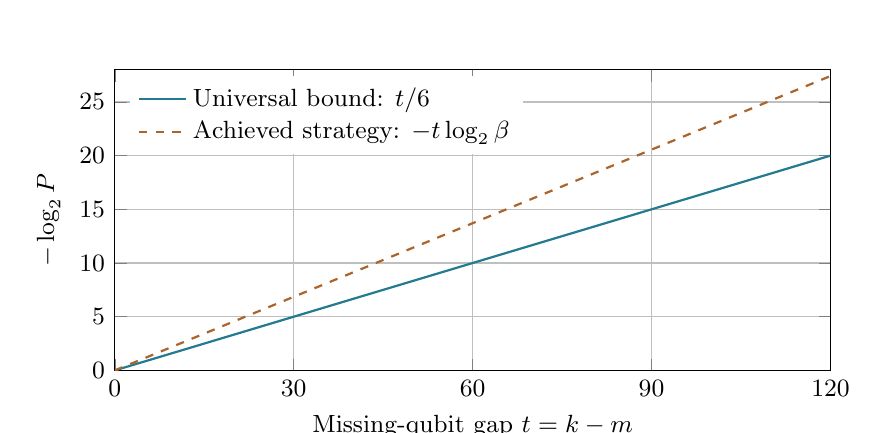
\begin{tikzpicture}
\begin{axis}[width=0.88\linewidth,height=54mm,xmin=0,xmax=120,ymin=0,ymax=28,
xlabel={Missing-qubit gap $t=k-m$},ylabel={$-\log_2 P$},
xtick={0,30,60,90,120},ytick={0,5,10,15,20,25},
tick label style={font=\small},label style={font=\small},grid=major,
legend style={font=\small,at={(0.02,0.98)},anchor=north west,draw=none,fill=white},
legend cell align=left]
\addplot[accent,thick,domain=0:120,samples=2]{x/6};
\addlegendentry{Universal bound: $t/6$}
\addplot[warm,thick,dashed,domain=0:120,samples=2]{0.228446696836388*x};
\addlegendentry{Achieved strategy: $-t\log_2\beta$}
\end{axis}
\end{tikzpicture}
\end{center}
\smallskip
The optimal value $-\log_2 P^*_{k,m}$ lies between the two lines; larger values mean smaller success probability.

\subsection{A finite comparison, with a precise scope}
An earlier uncertainty relation permits storage rates approaching one. To specialize it using only the memory dimension, one needs conditional min-entropy with a quantum first register. Its operator definition is
\[
2^{-H_{\min}(A\mid E)_\rho}
=\inf_{\omega_E\geq0}\{\Tr\omega_E:
\rho_{AE}\leq I_A\otimes\omega_E\}.
\]
Here $E$ denotes the available side information, and $\omega_E$ ranges over positive operators whose trace is unrestricted. When $A$ is classical this definition agrees with the guessing-probability definition above. The dimension bound gives $H_{\min}(A\mid CQ)\geq-\log_2d_Q\geq-m$. Indeed, Cauchy--Schwarz on a pure Schmidt decomposition gives $\rho_{AQ}\leq d_Q I_A\otimes\rho_Q$; averaging pure branches and classical records preserves this inequality. Thus $\omega_{CQ}=d_Q\rho_{CQ}$ is a feasible choice of trace $d_Q$. Substituting the resulting entropy bound into the earlier relation gives the particular sufficient bound
\[
H_{\min}(X\mid CQ\Theta)\geq\frac{k\gamma(-m/k)-1}{2},
\]
where $H_{\min}=-\log_2\pguess$ is the conditional min-entropy, and $\gamma(u)$ inverts
$h_2(a)+a-1$ on $0\leq a\leq1/2$. The binary entropy is
$h_2(a)=-a\log_2a-(1-a)\log_2(1-a)$, with $0\log_2 0=0$.
Writing $a=\gamma(-m/k)$ gives $t=k[h_2(a)+a]$. To reach $H_{\min}\geq\log_2(1/\delta)$, it suffices that $a\geq a_*=[1+2\log_2(1/\delta)]/k$. When $a_*\leq1/2$ and the gap is feasible, this yields $\lceil k[h_2(a_*)+a_*]\rceil$.

At $\delta=2^{-20}$, this gives the sufficient gaps below.
\begin{center}\small
\begin{tabular}{@{}rrr@{}}\toprule
Input size $k$ & This bound & Earlier specialization\\\midrule
$1{,}024$ & $120$ & $290$\\
$10{,}000$ & $120$ & $426$\\
$1{,}000{,}000$ & $120$ & $698$\\\bottomrule
\end{tabular}\end{center}
At a fixed target $\delta$, this earlier specialization retains a logarithmic block-size dependence. To see it, put $s=1+2\log_2(1/\delta)$, so $a_*=s/k$. For large $k$,
\[
k h_2(s/k)
=s\log_2(k/s)+s\log_2 e+O(s^2/k).
\]
Here $e$ is the base of the natural logarithm. Thus its sufficient gap grows as $s\log_2k+O_\delta(1)$, whereas \eqref{eq:gap} supplies a gap independent of $k$. The comparison fixes the two displayed unsmoothed guessing bounds and the dimension-only substitution. Additional state information or smoothing would define a different comparison.

\newsection{How classical interaction can supply the test}
\subsection{The extra preparation problem}
The ideal experiment supplies actual BB84 states. A verifier restricted to classical computation and communication uses a remote-state-preparation protocol instead: the verifier ends with hidden labels and a pass flag, and an honest quantum device ends with the corresponding qubits. Efficiency is measured in the security parameter $\lambda$. The preparation guarantee uses nonuniform quantum polynomial-time adversaries, simulators, and continuations: they may use advice depending on $\lambda$, but must remain within the specified polynomial resource bound. Its security inequalities hold for all sufficiently large $\lambda$ and polynomially bounded output length.

The imported construction relies on quantum hardness of learning with errors (LWE). At the level of notation, LWE involves noisy modular linear equations
\[
b=\langle a,s\rangle+e\pmod q,
\]
where $q$ is an integer modulus, $a,s$ are vectors over integers modulo $q$, and $e$ follows a specified error distribution. The construction imports a hardness assumption for its parameter family and quantum adversary class. That computational assumption supplies preparation security; the finite guessing theorem is an independent information-theoretic statement.

\subsection{The exact simulation interface}
For every efficient malicious preparation prover, the imported guarantee supplies an efficient simulator whose input is the ideal quantum BB84 state alone. It produces a simulated pass flag and the prover's output system. The simulator does not receive the classical hidden labels $x,\theta$.

For every efficient continuation and its acceptance test, the real and simulated probabilities of the joint event
\[
\{\text{preparation passes and continuation accepts}\}
\]
differ by at most $\eta_{\mathrm{prep}}$. The continuation may use the verifier's hidden labels to evaluate its test. The simulator's quantum input and the verifier's classical knowledge play different roles.

\begin{keybox}
The comparison is pass weighted: it directly bounds the joint event of preparation passing and the continuation accepting, without conditioning on a pass. The same simulator, chosen for the malicious preparation prover, must satisfy this comparison for every efficient continuation.
\end{keybox}

Honest preparation has a separate property: its joint state, including the verifier labels, is negligibly close in trace distance to the ideal BB84 source with a passing flag. Here trace distance is $\tfrac12\lVert\rho-\sigma\rVert_1$ for normalized states, with the ordinary trace norm $\lVert A\rVert_1=\Tr|A|$. It bounds the difference in any acceptance probability. This honest-state trace-distance property is separate from the computational comparison for malicious provers.

Under its polynomial quantum-hardness assumption, the construction supports polynomial-length output and inverse-polynomial simulation error using polynomially many rounds. The ideal inequality \eqref{eq:main} remains unconditional.

\newsection{Compose preparation with the storage bound}
\subsection{A reduction without conditioning on a pass}
Run the preparation protocol for $k$ output qubits. The verifier keeps its hidden strings and its flag. After the storage cut, send $\Theta$; accept exactly when preparation passed and the returned string equals $X$. On failed preparation the verifier may still send an independent dummy basis and always reject. The proof requires no early disclosure of the flag.

Fix an efficient adversary whose total retained quantum dimension at the cut is at most $2^m$. Let $E$ be its actual preprocessing and compression up to that cut. Use the imported simulation guarantee with the continuation that runs $E$, discloses the verifier's bases, runs the decoder, and checks the guessed string. It gives
\begin{align*}
P_{\mathrm{real\ accept}}
&\leq\eta_{\mathrm{prep}}
+P_{\mathrm{sim\ pass\ and\ correct}}\\
&\leq\eta_{\mathrm{prep}}+P_{\mathrm{sim\ correct}}.
\end{align*}
The simulator composed with $E$ is an encoder on ideal quantum BB84 inputs. As a map, $E$ has a charged quantum output register $Q$ of dimension at most $2^m$; applying it to the simulated state does not enlarge that register. Temporary workspace before the cut may be larger, but all quantum information accessible across the cut is charged. Classical transcripts and flags can be added to $C$. A discarded simulator environment is not later returned.

Giving arbitrary guesses to failed simulated branches makes a complete strategy covered by the ideal theorem. Thus
\[
P_{\mathrm{real\ accept}}\leq\min\{1,\eta_{\mathrm{prep}}+2^{-(k-m)/6}\}.
\]
The joint-event comparison keeps rare passing branches weighted by their actual probabilities throughout the argument.

\subsection{Allocate the error budget and state the efficient regime}
For target total false-acceptance probability $\varepsilon\in(0,1)$, it is sufficient to obtain $\eta_{\mathrm{prep}}\leq\varepsilon/2$ and choose
\begin{equation}\label{eq:k-choice}
k=m+\left\lceil6\log_2(2/\varepsilon)\right\rceil.
\end{equation}
For example, an ideal storage term at most $2^{-20}$ requires gap $120$. Total false acceptance at most $2^{-20}$ with equal allocation requires gap $126$ and preparation error at most $2^{-21}$. These numbers illustrate the algebraic allocation of the two error terms.

More precisely, let $m(\lambda)\geq0$ be integer valued, efficiently computable, and polynomially bounded, and let $p(\lambda)\geq1$ be a polynomial target. The imported construction supplies error $1/[2p(\lambda)]$ efficiently. Choosing
\[
k(\lambda)=m(\lambda)+\left\lceil6\log_2(2p(\lambda))\right\rceil
\]
yields a polynomial-round protocol with soundness at most $1/p(\lambda)$. Honest completeness is $1-\operatorname{negl}(\lambda)$ for ideal honest storage, where negligible means eventually smaller than every inverse polynomial. This finite storage estimate applies without a condition $m(\lambda)=\omega(\log\lambda)$. Efficient negligible-soundness compilation would require a preparation guarantee at the corresponding error scale; the imported efficient guarantee supplies the inverse-polynomial regime.

\newsection{Lists and tolerated wrong answers}
\subsection{Prove the list cost before changing the test}
In the ideal storage model, suppose a decoder output $y$ specifies a set $\mathcal L_y$ of at most $L\geq1$ candidate strings. Success means $X\in\mathcal L_y$. The list can depend on the basis and available records, but the unknown $X$ enters only through the decoder's actual information. For its POVM $\{M_y\}$, define
\[
F_x=\sum_{y:x\in\mathcal L_y}M_y.
\]
Then $0\leq F_x\leq I$ and $\sum_xF_x\leq LI$. Reuse $A_x=S^{-1/4}\sigma_xS^{-1/4}$ and set $B_x=S^{1/4}F_xS^{1/4}$. Now $0\leq B_x\leq S^{1/2}$, so
\begin{align*}
\sum_x\Tr B_x^2
&\leq\sum_x\Tr(B_xS^{1/2})
=\Tr\left(S\sum_xF_x\right)\leq L.
\end{align*}
The first inequality uses $\Tr[B_x(S^{1/2}-B_x)]\geq0$; positivity suffices even when the two operators do not commute. The same matrix Cauchy--Schwarz argument gives $P_{\mathrm{list}}^2\leq L\pgm$. On each pure branch, average its square root over the bases and use the rank estimate from Section~8. This gives $P_{\mathrm{list}}\leq\sqrt L(r/d)^{1/6}$. Averaging the branches yields
\begin{align}\label{eq:list}
P_{\mathrm{list}}&\leq\min\{1,\sqrt L(d_Q/2^k)^{1/6}\}\notag\\
&\leq\min\{1,\sqrt L\,2^{-(k-m)/6}\}\qquad(d_Q\leq2^m).
\end{align}
This proof applies separately to every basis, so the list can depend on the basis. Randomized list selection is included in the measurement outcome $y$. The list inequality is a direct scored-discrimination extension of the same square-root-measurement argument.

\subsection{Hamming tolerance changes the claim}
Allow at most $h$ wrong bits, where $h$ is an integer between zero and $k$. A returned string accepts all strings differing from it in at most $h$ positions: a Hamming ball of size
\[
V(k,h)=\sum_{j=0}^{h}\binom{k}{j}.
\]
Equation \eqref{eq:list} gives ideal cheating probability at most
$\min\{1,\sqrt{V(k,h)}\,2^{-(k-m)/6}\}$. With preparation error $\varepsilon/2$, the sufficient gap becomes
\[
k-m\geq3\log_2 V(k,h)+6\log_2(2/\varepsilon).
\]
For $h\leq k/2$, $V(k,h)\leq2^{k h_2(h/k)}$. A fixed positive error fraction therefore adds an extensive term to this sufficient estimate, which may become vacuous.

There is also a direct obstruction. A device storing $k-h$ designated qubits can recover those positions perfectly and guess the other $h$ arbitrarily. It always makes at most $h$ errors. For $k=1{,}000$ and allowance $h=10$, storing $990$ qubits guarantees acceptance. Thus the unmodified tolerant test cannot certify such a deficit with small false acceptance.

For the store-and-measure witness, an achieved tolerant success is
\[
\sum_{j=0}^{\min(h,t)}\binom tj(1-\beta)^j\beta^{t-j}.
\]
The obstruction concerns this acceptance rule and leaves other noise-tolerant certification protocols open.

\newsection{Erasures, honest noise, and preparation perturbations}
\subsection{The time of an erasure declaration matters}
Let $0\leq\ell\leq k$ be an integer. Write $P_{\mathrm{pre}}$ and $P_{\mathrm{post}}$ for ideal acceptance probabilities when erased positions are declared before or after basis disclosure. For a pre-basis declaration, condition on the erased set $S$ and earlier classical records in the delayed-measurement model. Discard the untested $A$ registers and put $k_S=k-|S|$. The surviving state may be arbitrary and mixed, but its remaining bases are independent and uniform. For $k_S\geq1$, the stronger theorem gives
\[
P_{\mathrm{pre}\mid S}\leq\min\{1,2^{-(k_S-m)/6}\}.
\]
For $k_S=0$ the upper bound is one. Since $k_S\geq k-\ell$, averaging over the declaration gives
\begin{equation}\label{eq:preloss}
P_{\mathrm{pre}}
\leq\min\{1,2^{-(k-\ell-m)/6}\}.
\end{equation}
Earlier measurement records may determine the declaration; the conditional bits need not be uniform.

If up to $h$ errors are also allowed, condition on the actual surviving length before applying the list bound. The conditional upper bound is
\[
\min\{1,\sqrt{V(k_S,\min\{h,k_S\})}\,2^{-(k_S-m)/6}\}.
\]
The radius is capped at $k_S$ because accepting $k_S$ or more errors accepts every surviving string. At $k_S=0$, $V(0,0)=1$ and the displayed minimum gives the trivial bound one. For a variable number of erasures, take the maximum over the permitted $k_S$: both the Hamming volume and the deficit depend on that length.

If instead the erased positions can be chosen after basis disclosure, a particular output with $\ell$ erasures accepts $2^\ell$ full strings. Applying the basis-dependent list bound gives
\begin{equation}\label{eq:postloss}
P_{\mathrm{post}}
\leq\min\{1,2^{\ell/2}2^{-(k-m)/6}\}.
\end{equation}
The output itself specifies the erased set, so its list size already accounts for that selection; there is no extra factor for the number of possible erased sets. With exactly $\ell$ erasures and at most $h$ wrong surviving bits, the list size is
\[
L=2^\ell V(k-\ell,\min\{h,k-\ell\}).
\]
With variable erasure count, take the largest permitted actual list size. These two guarantees distinguish a pre-basis commitment from an adaptive post-basis declaration. They are sufficient bounds for those acceptance rules, with their optimum constants left open.

\subsection{Completeness is a separate physical requirement}
If an honest device's recovered bits have independent error probability $e$, exact-string completeness is
\[
P_{\mathrm{honest\ correct}}=(1-e)^k.
\]
A fixed positive independent error rate therefore destroys completeness as $k$ grows. Without independence, the union bound still gives failure at most $\sum_i e_i$, where $e_i$ is the marginal probability of an error in bit $i$. To keep this failure contribution below $\eta$, it suffices that $\sum_i e_i\leq\eta$; uniform $e_i\leq\eta/k$ is one sufficient option.

An error-correction implementation would require its own physical resource accounting. The present ideal logical-qubit test supplies neither such an architecture nor a fixed-noise-rate threshold.

\subsection{A trace-distance perturbation is a different guarantee}
Let actual and ideal joint source states, including the verifier labels, be $\omega$ and $\omega_{\mathrm{id}}$, with $\xi=\tfrac12\lVert\omega-\omega_{\mathrm{id}}\rVert_1$. Any fixed acceptance test has an effect $0\leq M\leq I$, and
\[
\left|\Tr(M\omega)-\Tr(M\omega_{\mathrm{id}})\right|\leq\xi.
\]
Thus a specified physical source perturbation changes acceptance by at most $\xi$. The malicious-prover preparation guarantee instead compares computationally accessible joint pass-and-accept probabilities. Each guarantee must be used with its own premise.

\newsection{A conditional processing consequence in a noisy device}
\label{sec:noisy-processing}
\subsection{A different resource question, with an explicit chronology}
For this noisy-device application, use $k$ challenge qubits, total noisy physical width $n$, and $D$ noise rounds. The challenge length $k$ is the same as in the ideal theorem; $n$ and $D$ now count physical width and noise rounds, while $d_Q$ denotes retained quantum dimension in the ideal model. Width counts every persistent data, controller, syndrome and resource register.

Supply only $\ket X_\Theta$ for independent uniform $X,\Theta\in\{0,1\}^k$. Keep $X$ secret; disclose only $\Theta$ after all charged storage. The final decoder may depend arbitrarily on $\Theta$. Unconditional whole-string success is $p=\Pr[\widehat X=X]$, with aborts counted as failures.

Each round applies independent depolarization to every persistent register:
\[
\mathcal N_\gamma(A)=qA+(1-q)\frac I2\Tr A,
\qquad q=1-\gamma\in(0,1).
\]
The fixed circuit has free ideal Clifford operations and input-independent replacement resets. Every internal T/T-dagger is counted; other operations need a proved support-growth charge. Controllers obey these same rules: noisy counted bits do not make arbitrary feedback or data-dependent resets free. Arbitrary endpoints have no protected side channel across storage.

\subsection{Why a temporal cut is a quantum-plus-classical encoder}
Start one backward Pauli envelope at the full physical output before basis-dependent readout, with rank $M=2n$. At each cut, average earlier noise into a CPTP prefix. Every independent future-noise branch has tail-adjoint range in
\[
\mathcal A_V\simeq M_{2^s}\otimes\operatorname{Diag}_{2^c}\otimes I_G,
\qquad r:=\dim V=2s+c.
\]
The trace-preserving conditional expectation $\mathcal E_V$ is a CPTP map on the full physical memory. It factors as $\mathcal E_V=\mathcal J_V\mathcal F_V$: $\mathcal F_V$ changes to canonical coordinates, dephases the $c$-bit factor and traces out $G$, while $\mathcal J_V$ reinserts $I_G/\dim G$ and reverses the coordinate change. The tail satisfies $\mathcal S=\mathcal S\mathcal E_V$. Thus $\mathcal F_V$ composed with the prefix is a genuine $s$-qubit, $c$-bit encoder; composing $\mathcal J_V$ with the tail and readout reproduces the original outcome distribution.

Let $p_{b,t}$ be the actual endpoint decoder's success probability on the sampled channel. The finite guessing theorem and a separate finite-output count imply
\begin{equation}
p_{b,t}\le\min\{1,2^{(s-k)/6},2^{s+c-k}\}.
\label{eq:noisy-branch}
\end{equation}
For the last bound, fix a basis. The $2^k$ equiprobable inputs give output density matrices $\rho_x\le I$ on a space of dimension $2^{s+c}$, so any POVM has success at most $2^{s+c-k}$. Apply this count to the original normalized encoder, before the mathematical classical refinement used in the proof of the ideal theorem.

Noise flags select independent CPTP channels; they are proof aids, not postselection outcomes or device information. Branch-specific decoder optimization only raises the upper bound. Linearity gives $p=\E_b p_{b,t}$ at every primitive cut, on both sides of each gate and noise layer.

For $k\ge8$, the branch inequalities yield the useful uniform floor
\begin{keybox}
\begin{equation}
R_t:=\E_b\dim V_{b,t}\ge
a_p:=2k\frac{[p-2^{-k}]_+}{1-2^{-k}}.
\label{eq:noisy-floor}
\end{equation}
It is positive for every score above random guessing, including scores below one half.
\end{keybox}
Maximizing \eqref{eq:noisy-branch} at fixed $r$ gives $2^{r-k}$ up to $5k/6$, then $2^{(r-2k)/7}$ up to $2k$, and one thereafter. For $k\ge8$, both convex pieces lie below the chord from $(0,2^{-k})$ to $(2k,1)$; averaging proves \eqref{eq:noisy-floor}. For all $k\ge1$, finite-output counting gives the weaker floor $k[p-2^{-k}]_+/(1-2^{-k})$.

\subsection{The same floor controls gates in every interval}
For the backward envelope, a noise layer obeys $R'\le qR$, each T or T-dagger adds at most one binary generator, and free primitives add none. Put $\kappa=-\ln q$. Summing logarithmic changes at cuts with $R_t\ge a_p>0$ gives
\begin{equation}
m_T\ge
\frac{[D\kappa-\ln(2n/a_p)]_+}{\ln(1+1/a_p)}.
\label{eq:noisy-budget}
\end{equation}
Round the right side upward for the integer gate count. The weaker structural-charge form is $B\ge a_p[D\kappa-\ln(2n/a_p)]_+$ when a gate of charge $b_g$ can add at most $b_g$ generators and $B=\sum_gb_g$.

Every contiguous interval inherits the same floor. In \eqref{eq:noisy-budget}, use its own noise-layer and T counts and an entering expected-rank bound $M_I\le2n$. Interval noise is independent of the later suffix; boundary gates are assigned once. Gates outside a long interval supply only this finite reserve.

For example, $k=12,p=0.4,n=120,\gamma=0.01,D=2000$ gives $a_p\simeq9.59648$ and requires at least $171$ internal T/T-dagger gates. With the same score and width, every 700-round contiguous interval requires at least $39$ such gates by \eqref{eq:noisy-budget}. The scalar injection bound alone gives $37$. These are necessary processing budgets; their attainability and the device assumptions require separate evidence.

\subsection{What the recovery comparison and boundaries imply}
The recovery comparison remains informative even at scores at or below one half. For one complete branch channel, let $F_{\rm rec}$ be its optimum squared Bell-overlap recovery fidelity, $F_{\rm pg}\le F_{\rm rec}$ its pretty-good value, $u$ its average pretty-good guessing success, and $p_*\ge1/d$ its optimized guessing score. With $d=2^k$, established discrimination and recovery estimates give
\begin{align*}
p_*^2+\frac{(1-p_*)^2}{d-1}&\le u,\qquad F_{\rm rec}\ge p_*/d,\\
u&\le\tau_\ell+A_\ell F_{\rm pg},\qquad 0\le\ell\le k,\\
A_\ell&=\sum_{j=0}^{\ell}\binom kj(1-2^j\tau_\ell),
\end{align*}
where $\tau_\ell=2^{-\ell-1}$ for $\ell<k$ and $\tau_k=0$. The underlying spectral reduction writes $u=\sum_v\lambda_vw_v$, where $w_v\ge0$, $\sum_vw_v=1$, and $w_v\le F_{\rm pg}$. Its nonzero eigenvalues are $2^{-j}$ with multiplicities $2^j\binom kj$. Bounding all terms at or below $\tau_\ell$ by that threshold, then applying the cap to the excess, gives $u\le\tau_\ell+F_{\rm pg}\sum_{\lambda_v>\tau_\ell}(\lambda_v-\tau_\ell)$, which is the displayed estimate. At $\ell=0$ it gives $u\le(1+F_{\rm pg})/2$.

The actual branch score is at most $p_*$, and every branch satisfies $F_{\rm rec}\le\min\{1,2^{r-2k}\}$. These estimates reproduce \eqref{eq:noisy-floor} for every $k\ge8$ when applied branchwise \emph{before} averaging. Exact finite-rank checks also imply the weaker floor stated above for $1\le k\le7$. Thus these mean-rank floors and their gate or interval consequences already follow from the recovery route. The direct encoder factorization gives a short operational explanation; this comparison does not identify the optimal attainable score or exclude stronger bounds.

\subsection{Keeping the actual noise distribution gives a stronger budget}
The mean-rank comparison does not exhaust the specified noisy dynamics. For a fixed real $1<z\le2$, write $M_z(t):=\E_b z^{r_{b,t}}$ for the exponential moment of the common full-output envelope:
\begin{equation}
X_z(t):=\log_z\E_b z^{r_{b,t}},\qquad
\alpha_z:=\frac{\ln(1-q+qz^2)}{2\ln z}\in(0,1).
\label{eq:noisy-moment}
\end{equation}
This potential has terminal value $2n$. It uses the same counted registers, fixed primitives and mathematical noise flags as the preceding argument.

To see the contraction, choose $r$ binary pivot coordinates that identify a rank-$r$ envelope. Let $d_j\in\{0,1,2\}$ be the number of pivots on qubit $j$, so $\sum_jd_j=r$. If noise retains the site set $S$, then $\dim(V\cap W_S)\le\sum_{j\in S}d_j$. Independence and the inequality $(1-q+qz)^2\le1-q+qz^2$ imply
\[
\E[z^{r'}\mid V]\le\prod_j(1-q+qz^{d_j})
\le(1-q+qz^2)^{r/2}.
\]
Concavity of $x^{\alpha_z}$ gives $X_z'\le\alpha_zX_z$ at a noise layer. A T/T-dagger adds at most one to $X_z$; Clifford gates and input-independent resets cannot increase it. This retains information about the noise law that the mean-rank chord discarded, without assuming rank concentration.

Use the preceding discrimination and recovery estimates on the averaged channel to the full physical output. For $p\ge1/d$, define
\begin{equation}
F_0(p):=\max\left\{d^{-2},\frac pd,
\max_{0\le\ell\le k}
\frac{[g_d(p)-\tau_\ell]_+}{A_\ell}\right\},
\quad g_d(p)=p^2+\frac{(1-p)^2}{d-1}.
\label{eq:noisy-moment-recovery}
\end{equation}
For $p<1/d$, use $F_0=d^{-2}$ and a zero floor. Fix one CPTP recovery with squared Bell fidelity at least $F_0(p)$. At each cut, averaging its recovered future-noise branches gives the same fidelity. Every branch has fidelity at most $\min\{1,2^{r-2k}\}$. For $b=4^{-k}$ and $w=(F_0-b)/(1-b)$, the secant in the variable $z^r$ gives
\[
\min\{1,2^{r-2k}\}
\le b+(1-b)\frac{z^r-1}{z^{2k}-1}.
\]
Thus every primitive cut has the positive moment floor
\begin{equation}
X_z(t)\ge a_z^{\mathrm{rec}}:=\log_z\!\left[1+w(z^{2k}-1)\right]
\label{eq:noisy-moment-floor}
\end{equation}
whenever $p>2^{-k}$. At chance, $a_z^{\mathrm{rec}}=0$. The recovery is fixed across the proof branches and requires no knowledge of their flags.

The direct profile in \eqref{eq:noisy-branch} supplies another floor. Write $b_0=2^{-k}$, $H_k=2^{-k/6}$, $Y_t=z^{5k/6}$ and $Y_e=z^{2k}$. For $1<z\le2^{1/7}$, its two exponential pieces are convex in $Y=z^r$. Let $P_z(Y)$ be the concave polygon through $(1,b_0),(Y_t,H_k),(Y_e,1)$, constant after $Y_e$, omitting the middle point if it is below the endpoint chord. Then $p\le P_z(\E z^r)$ and
\[
a_z^{\mathrm{dir}}=\log_z P_z^{-1}(p).
\]
The inverse is linear in $p$ on each retained segment. If the middle point is omitted it is $1+(p-b_0)(Y_e-1)/(1-b_0)$. Otherwise it is $1+(p-b_0)(Y_t-1)/(H_k-b_0)$ below $H_k$, and $Y_t+(p-H_k)(Y_e-Y_t)/(1-H_k)$ above it. Set the floor to zero at or below chance. Use the larger available direct or recovery floor, denoted $a_z$. Both are positive above chance. The earlier comparison of mean-rank floors does not imply dominance over this refinement.

\begin{samepage}
Putting $\kappa_z=-\ln\alpha_z$, the same gate-balance argument gives
\begin{equation}
m_T\ge\left\lceil
\frac{[D\kappa_z-\ln(2n/a_z)]_+}{\ln(1+1/a_z)}
\right\rceil .
\label{eq:noisy-moment-budget}
\end{equation}
The companion discrete injection ledger applies with its contraction parameter replaced by $\alpha_z$ and floor replaced by $a_z$. Take the strongest result over $z$ and the earlier mean-rank bounds. For a contiguous interval, the entering reserve must bound $\log_z\E z^r$; $2n$ is safe. The earlier reserve on $\E r$ alone is insufficient for this substitution.
\end{samepage}

At fixed positive score, both $b_0$ and $H_k$ decay exponentially. Choosing $\ln z=1/\sqrt{k}$ for large $k$ yields $a_z=2k-O_p(\sqrt{k})$ and $\alpha_z=q+O_q(k^{-1/2})$. The recovery bridge also reaches $a_z=2k-o(k)$, using its polynomial lower bound on $F_0(p)$. If $q\in(0,1)$ is fixed, $n\ge k$, $D\to\infty$, and $\ln(n/k)=o(D)$, the discrete ledger therefore implies
\begin{equation}
m_T\ge(2-o(1))\,k\,\frac{1-q}{q}\,D.
\label{eq:noisy-moment-asymptotic}
\end{equation}
The previous chord gives leading coefficient $2p$ under the same conditions. The moment argument strengthens the fixed-score dependence while retaining the weak-noise order $k\gamma D$. It supplies a necessary rate along feasible families, without constructing a memory or determining its optimum physical cost.

The analytic polygon can be sharpened by combining all available bounds at each integer pair $(s,c)$. For $k=12$, a rational certificate checks all 169 pairs with $0\le2s+c\le24$, using the direct, recovery and output-dimension caps and the established classical cap $\beta^{12}$ for $s=0$, where $\beta=(1+1/\sqrt2)/2$. At $z=27/25$, the concave polygon through $(1,1/4096),(z^{11},1/4),(z^{24},1)$, constant afterward, majorizes each branch cap. The classical bound follows from the Gram-matrix row-sum estimate for selected product-BB84 vectors.

The three-input bound also survives this composition. For $k=3,s=1$, the branch cap is $C_3$ regardless of the allowed classical dimension. At $r=4,s=1,c=2$ it is smaller than the previous normalized recovery cap. For $z=27/25$, a rational concave majorant of the improved integer profile has knots
\[
(1,1/8),\quad(z^2,1/2),\quad(z^3,311/500),\quad
(z^4,93/125),\quad(z^6,1).
\]
Exact rational slope and cap checks certify this polygon. Thus $\E z^r\le z^4$ forces $p\le93/125=0.744$. At score $p=3/4$, the moment floor is at least $\log_z[z^4+3(z^6-z^4)/128]>4$. This is a finite interface improvement; it changes neither the $k=12$ example nor the general exponent.

The four-input refinement also survives averaging. At $k=4$ and $z=27/25$, combine $C_4$ on $s=1$ branches with the output-dimension, classical dimension-lifting, normalized recovery and hypercontractive collision bounds. A certified concave polygon has knots
\[
(1,1/16),\qquad(z^3,1/2),\qquad(z^6,789/1000),\qquad(z^8,1),
\]
and equals one afterward. All 25 integer pairs $(s,c)$ with $0\le2s+c\le8$ and the decreasing slopes are checked exactly. Its value at $z^5$ is $6951/10145<7/10$, so score $p=7/10$ implies
\[
X_z\ge\log_z\!\left[z^3+\frac{200}{289}(z^6-z^3)\right]
=5.1476692298\ldots>5.
\]
The specified prior caps permit $7/10$ at rank five with $(s,c)=(1,3)$, since their smallest collision cap is $1/2$ and $g_{16}(7/10)=62/125<1/2$. This strict improvement compares proved outer profiles, without claiming that the previous profile is attainable or the new majorant optimal.

For the earlier example $k=12,p=0.4,n=120,q=0.99$, it gives $M_z\ge(4z^{11}+z^{24})/5$, $a_z\simeq14.84082963$ and $\alpha_z\simeq0.99072498$. Certified logarithm bounds make the individual-gate requirement at least $244$ for $D=2000$, compared with $171$ from mean rank. Every 700-round contiguous interval with moment reserve at most $240$ requires at least $58$ such gates, compared with $39$. The interval bound uses its own moment reserve, and both numbers are necessary conditions rather than physical feasibility or optimality claims.

\subsection{A finite and asymptotic decay guarantee}
The companion processing analysis owns the ledger and its inversion. The shared consequence is independently stated here. For $1<z\le2^{1/7}$ put $\alpha=\alpha_z$, $M=2n$, and, for $D\ge1$, define
\[
U_z=\min\left\{M\alpha,\;
\min_{1\le l\le D}\frac{\alpha(m_T+M\alpha^{l-1})}{1+(D-l)(1-\alpha)}\right\}.
\]
The direct profile gives $X_z\ge[2k+\log_zp]_+$. The scalar injection inequalities rearrange to upper-bound that floor by every expression defining $U_z$, yielding
\[
p\le\min\{1,z^{U_z-2k}\},\qquad
-\ln p\ge(\ln z)[2k-U_z]_+.
\]
For $D=0$ use $U_z=M$; for $p=0$ use $-\ln0=+\infty$. The initial-width term is retained, and any proved nondecreasing concave profile gives the stronger finite form $p\le P_z(z^{U_z})$. At $k=12,n=120,q=0.99,z=27/25,D=2000,m_T=200$, the certified profile gives $p\le0.310300082242$; the simple exponential bound gives $p\le0.418535080865$.

Fix $q\in(0,1)$ and finite $\rho\ge0$. Along any family with $k,D\to\infty$, $n\ge k$, $\ln(n/k)=o(D)$ and $\limsup m_T/(kD)\le\rho$,
\[
\liminf\frac{-\ln p}{k}\ge
E_q(\rho):=\sup_{1<z\le2^{1/7}}(\ln z)
\left[2-\rho\frac{\alpha_z}{1-\alpha_z}\right]_+.
\]
For fixed $z$, choose $l=1+\lceil\ln(2n/k)/(-\ln\alpha_z)\rceil=o(D)$, leaving initial allowance at most $k$. The displayed limit follows from the finite formula, followed by the supremum over fixed $z$. Since $\alpha_z>q$ and $\alpha_z\to q$ as $z\downarrow1$, the exponent is positive exactly when $\rho<2(1-q)/q$. The right endpoint is allowed and the continuous left-endpoint value is zero. This is a necessary-rate decay statement, not an achievable processing capacity.

The full generating-function transition gives a stronger exponent. Put
\[
\phi_j(\lambda)=\frac12\ln\bigl(1+q^j(e^{2\lambda}-1)\bigr),\qquad
A(\lambda)=\min\{2\lambda,(\ln2+5\lambda)/6,\ln2\}.
\]
Then $p\le e^{-kA(\lambda)}M_{e^\lambda}$, and summing over the last $T=D-L+1$ backward post-noise cuts gives
\[
\frac{-\ln p}{k}\ge\left[A(\lambda)-
\frac{2n\sum_{d=L}^D\phi_d(\lambda)+m_T\sum_{j=1}^T\phi_j(\lambda)}{kT}\right]_+.
\]
Each gate contributes at distinct positive noise ages, so this bound covers arbitrary prescribed schedules. Removing the initial width transient under the same growth assumptions proves
\[
\liminf\frac{-\ln p}{k}\ge\mathcal E_q(\rho):=
\sup_{0\le\lambda\le\ln2}\left[A(\lambda)-\rho\sum_{j\ge1}\phi_j(\lambda)\right]_+.
\]
The convergent series admits explicit geometric tail bounds. This exponent strictly improves $E_q$ below the same critical rate $2(1-q)/q$. At zero normalized processing rate, $\mathcal E_q(0)=\ln2$, matching the exponent of uniform guessing. It does not identify an achievable positive processing capacity.

\subsection{A reliability logarithm from complete envelope extinction}
A fixed above-chance score also limits the accumulated probability that the noisy memory loses \emph{all} input dependence. This supplies a continuing-processing bound even when the challenge length stays small. Keep the same independent replacement-noise coupling and full-output envelope. For $D\ge1$ and $2^{-k}<p<1$, put
\[
\delta_p=\frac{1-p}{1-2^{-k}},\qquad
b_p=1-\delta_p=\frac{p-2^{-k}}{1-2^{-k}}.
\]
The resulting necessary count is
\begin{equation}
m_T\ge\left\lceil\left[
\frac{\gamma D b_p}{\ln(1/\gamma)}
\left[\ln\frac{D b_p}{\delta_p}\right]_+-2n
\right]_+\right\rceil.
\label{eq:noisy-reliability}
\end{equation}
The finite subtraction is the terminal width reserve. This bound can be combined with the earlier rank and moment budgets; it does not assert that each finite relaxation dominates all the others.

For the proof, choose the backward envelope updates so that zero remains zero. Clifford gates and resets already have this property. At a T/T-dagger gate, retain $V$ if all its labels commute with the gate's Pauli axis $w$, and otherwise use $V+\langle w\rangle$. This preserves the support condition and rank-growth charge at most one. Always adding the axis, even to the zero space, would create an artificial resurrection and would not support the argument.

Let $r_j$ be the rank immediately before the $j$th backward noise layer, and let $S_j$ indicate $r_j>0$. A rank-$r_j$ binary space has $r_j$ pivot coordinates that determine every vector. These coordinates occupy at most $r_j$ physical qubits. Replacement of all these qubits annihilates the surviving space, because the corresponding restriction is injective. Current noise is independent of the sampled suffix that determines $V$, so this event has conditional probability at least $\gamma^{r_j}$. The flags remain proof variables, unavailable to the physical circuit.

A zero envelope gives a tail-adjoint range consisting only of scalar operators. The full physical output is therefore independent of the supplied input. Subsequent readout may depend on the disclosed basis, but it cannot correlate its guess with the uniformly hidden string. Such a branch scores at most $2^{-k}$, including any aborts as failures. If $e$ is the eventual extinction probability, unconditional averaging gives
\[
p\le(1-e)+2^{-k}e,\qquad e\le\delta_p.
\]
Because zero is absorbing, first extinction at different noise layers gives disjoint events. Any extinctions caused by resets consume additional probability and cannot invalidate the upper budget. Consequently,
\[
\sum_{j=1}^D\E[S_j\gamma^{r_j}]\le\delta_p,
\qquad A:=\sum_{j=1}^D\Pr(S_j=1)\ge D b_p.
\]
Apply Jensen to $e^{-r\ln(1/\gamma)}$ with the alive cut-time weights normalized by their total mass $A$. Since $r_j=0$ when $S_j=0$,
\[
\delta_p\ge A\exp\!\left[-\frac{\ln(1/\gamma)}{A}
\sum_{j=1}^D\E r_j\right].
\]
Combine this with nonnegativity. The function $x[\ln(x/\delta_p)]_+$ is nondecreasing for positive $x$, so
\[
\sum_{j=1}^D\E r_j\ge
\frac{A}{\ln(1/\gamma)}\left[\ln\frac{A}{\delta_p}\right]_+
\ge\frac{D b_p}{\ln(1/\gamma)}
\left[\ln\frac{D b_p}{\delta_p}\right]_+.
\]
Each noise layer loses at least $\gamma\E r_j$ expected rank, free processing cannot add rank, and all T/T-dagger increases sum to at most $m_T$. Telescoping from rank $2n$ therefore gives $m_T\ge\gamma\sum_j\E r_j-2n$, proving \eqref{eq:noisy-reliability}.

A sharper finite theorem keeps the symplectic information and the exact survival product. Let $a=a_k(p)$ be the all-cut rank floor: use $a_p$ in \eqref{eq:noisy-floor} for $k\ge8$. For $1\le k\le7$, with $H=2^{-k/6}$ and $t_0=5k/6$, the inverse of the concave polygon through $(0,2^{-k}),(t_0,H),(2k,1)$ gives
\[
a_k(p)=\begin{cases}
t_0(p-2^{-k})/(H-2^{-k}),&2^{-k}<p\le H,\\
t_0+(2k-t_0)(p-H)/(1-H),&H\le p<1.
\end{cases}
\]
Define
\[
a_s(p)=k\left[\frac{p-2^{-k/6}}{1-2^{-k/6}}\right]_+,\qquad
L_\gamma(D,b)=\frac{b}{\ln(1/\gamma)}\ln\frac1{1-b^{1/D}}.
\]
Then
\begin{equation}
\boxed{m_T\ge\left\lceil\left[
\gamma D\max\{a,a_s(p)+L_\gamma(D,b_p)\}+a-2n
\right]_+\right\rceil.}
\label{eq:noisy-reliability-sharp}
\end{equation}
The quantum-factor floor is derived from the BB84 branch bound, independently of any Bell-fidelity premise. Indeed its secant gives
$\min\{1,2^{(s-k)/6}\}\le2^{-k/6}+(1-2^{-k/6})s/k$, so averaging implies $\E s\ge a_s(p)$. This extra floor vanishes when $p\le2^{-k/6}$.

For the sharper hazard, a rank-$r$ Pauli space of symplectic rank $2s$ has an injective coordinate set on at most $r-s$ physical sites. Choose a nondegenerate $2s$-dimensional subspace with generator matrix $H$. In the Cauchy--Binet expansion of $\det(H\Omega H^T)=1$ over $\mathbb F_2$, coordinate subsets not invariant under swapping each local $X,Z$ pair cancel in pairs. A remaining nonzero minor supplies $s$ complete pairs. Extend them to $r$ independent columns with at most $r-2s$ more sites. Erasing these sites annihilates the envelope, with conditional probability at least $\gamma^{r-s}$.

Let $t_j=\E[r_j-s_j\mid r_j>0]$. Conditioning on survival and applying Jensen to the fresh layer gives conditional survival probability at most $1-\gamma^{t_j}$. Operations between layers cannot resurrect zero. Thus
\[
b_p\le\prod_{j=1}^D(1-\gamma^{t_j}).
\]
The decreasing convex function $-\ln(1-e^{-\lambda t})$, with $\lambda=\ln(1/\gamma)$, gives
$\sum_jt_j\ge D\lambda^{-1}\ln[1/(1-b_p^{1/D})]$.
Each incoming survival probability is at least $b_p$, hence
$\sum_j\E(r_j-s_j)\ge D L_\gamma(D,b_p)$.
Add the independently proved floor $\E s_j\ge a_s(p)$, compare with $\E r_j\ge a$, and retain the exiting rank $\E r_{\rm end}\ge a$ in the telescope. This proves \eqref{eq:noisy-reliability-sharp}.

For a contiguous interval, replace $D,m_T,2n$ by $D_I,m_{T,I},M_I$ in the sharpened formula, retaining the same global score-derived floors and the actual propagated suffix envelope. The universal entering bound $M_I=2n$ is safe. The suffix is independent of fresh interval noise; successive hazards need not be independent. Assign boundary gates once to the chosen primitive cuts.

For fixed $k$, fixed $\gamma>0$ and fixed nonchance score, $n=O(\ln D)$ now forces $m_T=\Omega(D\ln D)$. Thus a constant rank floor at a single cut misses a reliability cost accumulated over a long storage period. In the companion construction range $0<\gamma\le1/20$, this order matches its reference-stable Tanner construction at logarithmic width and fixed error target. The comparison fixes noise strength; the coefficient $1/\ln(1/\gamma)$ does not give uniform weak-noise sharpness. The ideal guessing exponent and finite-input upper caps remain unchanged.

At $p=1$, positive noise duration and finite physical width are impossible: complete replacement of the whole register has positive probability and leaves only chance success. At or below chance, the discard-and-guess strategy remains consistent with zero processing. Nothing in this inference tests the assumed noise or controller restrictions or compiles the separate preparation protocol into the charged circuit.

\subsection{The coherent construction's matching regime}
The companion also owns the constructive processing theorem. It compiles an inherited good Tanner-code decoder, run for a fixed number of parallel iterations, into the allowed Clifford+T circuit. Every local minimum, comparison, tie choice and update is a fixed Boolean function on a constant-size neighborhood. Hardwired incidence connections require no adaptive address machine. Reversible Boolean evaluation, controlled Pauli correction and inverse evaluation cost $O(N)$ prescribed T slots and $O(N)$ total scratch for a data block of length $N$. Scratch is reset before each epoch and never retains a protected record.

The coherent circuit implements exactly $\sum_sP_{f(s)}\Pi_s\omega\Pi_sP_{f(s)}^\dagger$, also with an arbitrary reference. A constant-iteration residual contraction keeps both CSS components in a region whose combined representatives have weight below half the code distance. Current syndrome alone suffices. Independent depolarizing batches have correlated X/Z components on each site, so reliability uses their separate binomial tails and a union bound. Bounded multiplicative gaps in the available code lengths allow arbitrary payloads and error targets by padding within the free endpoints. A fixed number of five-qubit concatenation levels on every outer data position reduces fresh errors into this correctable region. Inner decoding, outer correction and reencoding use fixed circuits, and old outer logical Paulis leave the inner syndrome unchanged. Fresh inner residual labels are independent across outer positions and may have correlated X/Z components. The level depends only on the Tanner family. The combined construction gives, throughout $0<\gamma\le1/20$,
\[
\begin{gathered}
n=O\!\left(k+\ln\frac{J_+}{\epsilon}\right),\qquad m_T=O(nJ),\qquad J=O(\gamma D+1),\\
\tfrac12\lVert\Lambda-\mathrm{id}\rVert_\diamond\le\epsilon,
\qquad J_+=\max(1,J).
\end{gathered}
\]
Here $n$ counts data, syndrome and all workspace. The fixed constants are potentially enormous and the inner code increases them further. If $k=\Omega(\ln(J_+/\epsilon))$ and $\gamma D\to\infty$, the earlier payload converse already matches this processing order. The extinction-based fidelity converse extends fixed-noise matching to every payload scaling. For fixed $0<\gamma\le1/20$, fixed $\epsilon_0<1/2$, any $0<\epsilon\le\epsilon_0$ and widths $n\le C[k+\ln(D/\epsilon)]$, sufficiently large $D$ requires $m_T=\Omega_\gamma(D[k+\ln(D/\epsilon)])$. Combining the two lower bounds uses their shared cumulative rank, whose payload floor supplies the $k$ term and whose survival requirement supplies the reliability logarithm. A sufficiently large constant width factor permits this construction and gives the matching upper order. This is an optimum-order statement in the specified width class, not over arbitrarily large memories. It proves neither a numerical optimum nor a physical threshold with faulty gates or locality constraints. No preparation wrapper is automatically compiled into this processing theorem.

The same comparison determines the minimum width itself. For fixed $0<\gamma\le1/20$ and $0<\epsilon\le\epsilon_0<1/2$, the minimum permitted width for Bell infidelity or half-diamond error at most $\epsilon$ is
\[
n_{\min}=\Theta_{\gamma,\epsilon_0}\bigl(k+\ln(D/\epsilon)\bigr),\qquad k,D\ge1.
\]
The payload lower bound $n\ge k$ follows from the Schmidt-number cap $F_{\rm e}\le2^{n-k}$. With $b=1-\epsilon/(1-4^{-k})$, complete-register replacement gives the exact additional lower bound
\[
n\ge\left\lceil\frac{\ln[1/(1-b^{1/D})]}{\ln(1/\gamma)}\right\rceil.
\]
Since $b\ge1-4\epsilon_0/3>0$, this is uniformly logarithmic in $D/\epsilon$, up to fixed additive constants absorbed by the payload bound. The reference-stable Tanner construction supplies the matching upper order. Thus the processing order above holds within a sufficiently large fixed factor of minimum width; an arbitrary smaller factor need not fit the construction. For $D=0$, minimum width is exactly $k$ in this error range. These are transmission-fidelity statements, rather than minimum-width claims for every nonchance guessing score.

At chance, discarding the challenge and guessing needs zero processing. Full-register replacement gives
\[
p\le2^{-k}+(1-2^{-k})(1-\gamma^n)^D
\]
regardless of gates. Fixed width cannot sustain a fixed above-chance score indefinitely. Success does not verify noise, controller or side-channel premises. The remote-preparation reduction of Section~11 needs a separate model- and resource-preserving argument to compile this witness.

\newsection{Resources and interpretation}
\subsection{Which resource improves}
The earlier polynomial-hardness construction used $\lceil9.1m\rceil$ honest stored qubits in its stated asymptotic regime. In the same preparation framework, the finite bound replaces that multiplicative persistent-storage overhead by the additive gap \eqref{eq:k-choice}. The protocol wrapper and preparation construction supply the classical-verifier realization. Their separate constant-round variants use stronger assumptions and address a different resource tradeoff.

\begin{center}\small
\renewcommand{\arraystretch}{1.13}
\begin{tabularx}{\linewidth}{@{}p{42mm}X@{}}\toprule
Resource & What is counted \\\midrule
Honest persistent storage & $k$ ideal logical qubits through the waiting period.\\
Adversarial storage & Joint dimension of all later-accessible quantum systems at the cut, at most $2^m$.\\
Classical records & Unbounded in the ideal theorem; efficiently generated in the computational protocol.\\
Preparation and workspace & Imported preparation work and temporary ancillas; polynomial in its supported regime, with no optimized total-cost estimate here.\\
Communication and rounds & Classical interaction inherited from preparation; polynomially many rounds in the stated polynomial-hardness regime.\\
Readout and timing & Honest product-basis readout and classical checking; waiting duration is specified externally, with no new timing-enforcement mechanism.\\
Physical protection & Any additional physical qubits used for error correction remain physical quantum storage.\\\bottomrule
\end{tabularx}
\end{center}

No free state-loading oracle or quantum random-access memory is assumed. The ideal source is an explicit quantum input resource; its classical realization pays for the imported preparation protocol.

\subsection{What supports the claims}
The ideal result follows from the analytical chain in Sections~4--8, using the standard tensor-power norm theorem as its substantial mathematical input. Section~11 supplies the separate computational reduction under its cryptographic assumption. Finite matrix checks test the intermediate identities and normalization conventions against those analytical expressions. The three-, four- and five-input collision certificates use inherited positive two-copy shadow expressions, Pauli-weight bounds and exact algebra. The four- and five-input optima and their finite-alphabet conversions are certified separately. The three- and four-input moment polygons are checked at every permitted integer rank. The collision-route limitation follows from the explicit type construction and entropy expansion, rather than extrapolation of small instances. The direct-discrimination follow-up checks complete primal/dual matrices exactly for two fixed encoders and proves a separate diagonal-dual limitation analytically. Its finite optimal-decoder certificates are not upper bounds over arbitrary encoders.

The noisy-processing checks compare the explicit quantum-plus-classical factorization with the Pauli-algebra projection and verify the resulting endpoint probabilities. Independent moment checks enumerate all subspaces at widths one through three and certify the pivot, noise and gate inequalities; exact logarithm enclosures check the finite moment-budget comparison. The companion checks additionally certify the finite inverse ledger and its one-variable exponent optimization. The extinction theorem combines a paired symplectic-pivot hazard, a conditional survival product, the score-specific quantum-factor floor and cumulative-rank balance with the exiting rank retained; finite subspace, schedule and exact numerical checks supplement the written arguments. These checks do not test a physical device's noise or controller assumptions.

An accepted run is not a deterministic measurement of a device's qubit count. Soundness bounds every dimension-limited strategy in the ideal model; the compiled protocol covers the efficient adversaries in its imported assumptions. A low-memory device can occasionally pass. Claims based on repeated runs must account for their joint strategy and information across cuts rather than assuming independent trials without justification.

\end{document}

